\chapter{Modelowanie warunków propagacji}
\section{Motywacja}
Kiedy proces implementacji osiąga pewien stopień zaawansowania nadchodzi czas testowania. 
Oznacza to sprawdzenie projektu pod kątem dostępnych funkcjonalności. 
Prototyp poddany zostaje testom, aby upewnić się czy nie posiada poważnych wad. 
Komercyjne ścieżki rozwoju produktu dopuszczają równoległy proces weryfikacji zarówno u producenta jak u klienta, aby lepiej dostosować się do jego potrzeb \cite{product_dev}. 
System odbiornika tworzony jest dla celów edukacyjnych, dlatego testy zostaną wykonane wyłącznie przez autora projektu. 

W tym rozdziale duży nacisk położony jest na poznanie sygnału, który dociera do odbiornika. 
Odtworzone zostaną warunki pracy odbiornika poprzez spreparowanie sygnału i poddanie go działaniom zjawisk występujących w kanale radiowym. 
\section{Strategia}
Założenia projektowe nie określają jasno wymogów jakościowych i wydajnościowych pracy, a przyjęta strategia weryfikacji ma charakter eksperymentalny. 
Jako pierwsza przetestowana zostanie zdolność odbiornika do eliminacji zakłóceń pojedynczej częstotliwości. 
Scenariusz pokazany na Rysunku \ref{cwmodel} zakłada, że w kanale transmisyjnym sygnał użyteczny silnie interferuje z falą sinusoidalną. 
Dodatkowo występuje nieznaczny dryft częstotliwości sygnału zakłócającego w czasie.
Druga próba to modelowanie kanału jako filtra liniowego o zmiennej w czasie odpowiedzi impulsowej. (Rysunek \ref{mpathmodel})
Pozwoli to na przetestowanie odbiornika w warunkach zakłóceń związancych z propagacją wielodrogową \cite{indoor_ch_model}.

\begin{figure}[ht]
\centering
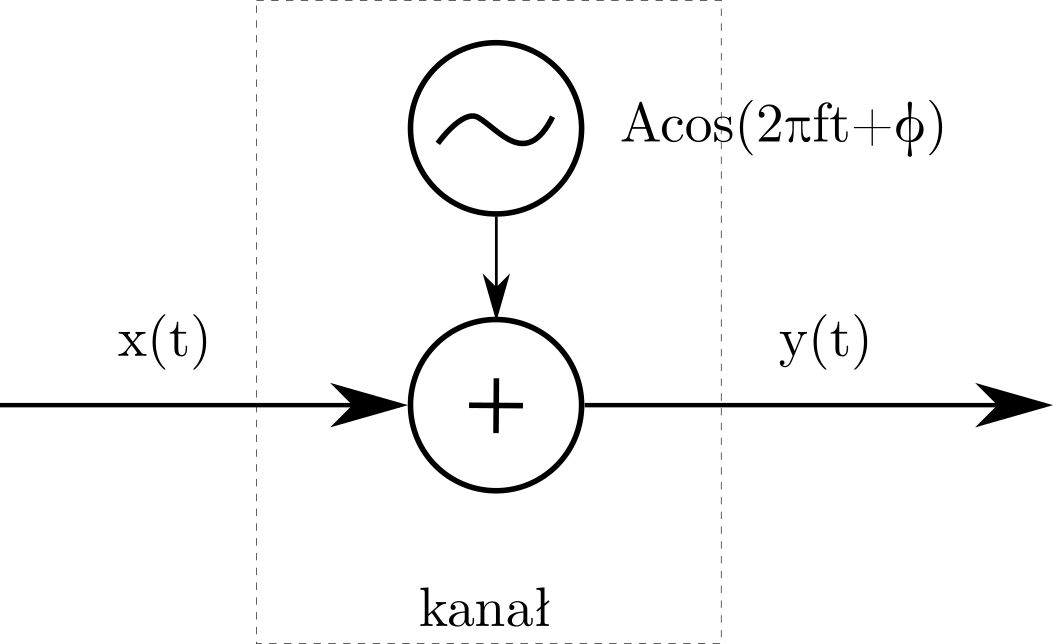
\includegraphics[scale=1.5]{ch_model1.png}
\caption{Model kanału z zakłóceniem pojedynczej częstotliwości}
\label{cwmodel}
\end{figure}

\begin{figure}[ht]
\centering
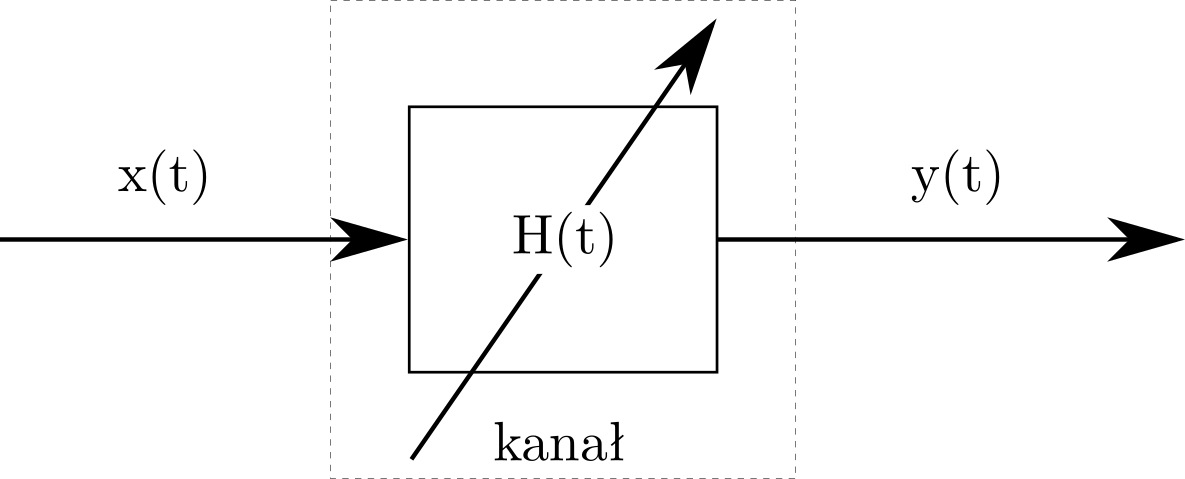
\includegraphics[scale=1.5]{ch_model2.png}
\caption{Model kanału w propagacji wielodrogowej}
\label{mpathmodel}
\end{figure}
\section{Symulowanie zakłóceń}
\subsection{Sygnał sinusoidalny}
Źródłem zakłóceń w postaci sygnałów sinusoidalnych mogą być radary dużych mocy, których częstotliwości harmoniczne zachodzą na pasmo użyteczne innych systemów \cite{Haykin:2004:MWC:984217}.
Głównym powodem testowania działania odbiornika dla tego rodzaju zakłóceń jest popularna aplikacja, w której algorytm LMS jest w stanie śledzić pulsację wolnozmiennego sygnału i adaptacyjnie dostosowywać nastawy filtra \cite{Haykin:1996:AFT:230061}.
Źródłem sygnału będzie blok \texttt{Signal Source}, który jako parametr przyjmuję amplitudę i~częstotliwość fali. 

\subsection{Zjawisko wielodrogowości}
Występuje wtedy, gdy sygnał z nadajnika, odbity od elementów otoczenia, dociera do odbiornika więcej niż jedną drogą. 
Czas propagacji jest różny dla różnych dróg sygnału. 
Tym samym każdy sygnał dociera do odbiornika opóźniony lub przyspieszony. 
Fale interferują, wzmacniają się lub osłabiają. 
W określonym czasie przy zachowaniu rozmieszczenia elementów otoczenia, nadajnika i odbiornika, kanał radiowy można traktować jako filtr o odpowiedzi impulsowej $h(t)$ \cite{Haykin:2004:MWC:984217}. 

Jako model kanału z propagacją wielodrogową posłuży blok \texttt{Channel Model}. 
Istotnym argumentem wejściowym dla bloku jest wektor współczynników o długości $M$. 
Współczynniki przyjmują wartości z zakresu $w_i = [0,1]$, gdzie 0 to brak tłumienia, a dla 1 tłumienie $\to \infty$. 
Charakterystyka kanału określona jest w przedziale $[-\frac{f_s}{2} + f_c,\frac{f_s}{2} + f_c]$, gdzie $f_s$ to częstotliwość próbkowania, a $f_c$ częstotliwość nośna sygnału. 
Pasmo kanału dzielone jest na odcinki o szerokości $\frac{f_s}{M}$. 
Za tłumienie na każdym z $M$ odcinków odpowiada jeden współczynnik.
Wartości współczynników powiązane zostały z suwakami do regulacji z panelu graficznego dla lepszej kontroli charakterystyki.

W celu zbadania charakterystyki, na wejście podłączono dwa sygnały szumu białego. 
Na Rysunku \ref{channel_model} przedstawiono widma tych sygnałów po przejściu przez blok kanału radiowego. 
Jedno wejście nie zostało poddane filtracji dla zachowania punktu odniesienia. 
W drugim, część częstotliwości została stłumiona przez zastosowanie filtra o regulowanych współczynnikach.

Efektem takich zakłóceń mogą być błędy w procesie decyzyjnym odbiornika, które prowadzą do zmniejszenia efektywnej przepustowości kanału. 

\begin{figure}[ht]
\centering
\caption{Charakterystyka częstotliwościowa kanału radiowego}
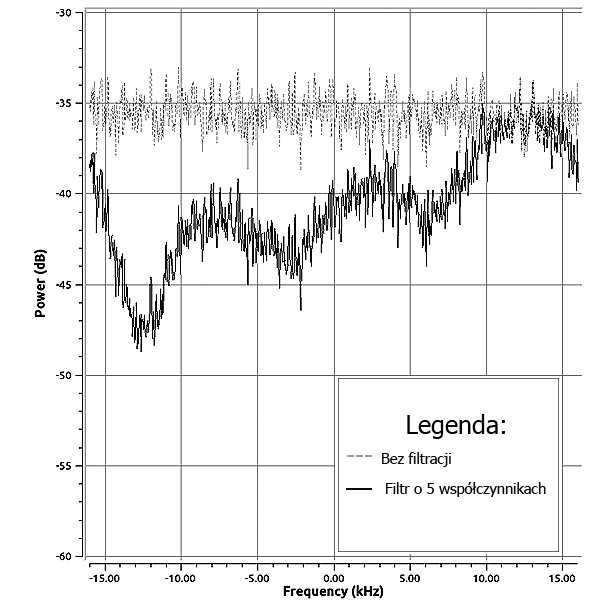
\includegraphics[scale=1.5]{ch_model3.png}
\label{channel_model}
\end{figure}

\section{Podsumowanie}
Przedstawione zostały dwa rodzaje zakłóceń, które posłużą do przeprowadzenia testów na odbiorniku.
\begin{enumerate}
\item Sygnał pojedynczej częstotliwości, pochodzący ze źródeł sąsiednich systemów telekomunikacyjnych.
\item Zwielokrotnienie tego samego sygnału w odbiorniku powodowane zjawiskiem propagacji wielodrogowej.
\end{enumerate}
